% Compile with: pdflatex Agent_Hackathon_Intro.tex (twice for refs)
\documentclass[aspectratio=169,10pt]{beamer}

\usepackage[T1]{fontenc}
\usepackage{lmodern}
\usepackage{amsmath,amssymb}
\usepackage{tikz}
\usetikzlibrary{arrows.meta, positioning, shapes.geometric, calc, fit, backgrounds}
\usepackage{listings}
\usepackage{xcolor}

% ---------- Penn colors ----------
\definecolor{pennblue}{RGB}{1, 31, 91}
\definecolor{pennred}{RGB}{153, 0, 0}
\definecolor{pennlight}{RGB}{240, 244, 250}
\definecolor{codebg}{RGB}{248, 248, 248}
\definecolor{codegray}{RGB}{100, 100, 100}

% ---------- Theme ----------
\usetheme{default}
\setbeamercolor{structure}{fg=pennblue}
\setbeamercolor{frametitle}{fg=pennblue}
\setbeamercolor{title}{fg=pennblue}
\setbeamercolor{author}{fg=black}
\setbeamercolor{institute}{fg=codegray}
\setbeamercolor{section in toc}{fg=pennblue}
\setbeamertemplate{navigation symbols}{}
\setbeamertemplate{frametitle}{%
  \vskip0.4em\hspace{0.5em}\usebeamercolor[fg]{frametitle}\large\bfseries\insertframetitle%
  \vskip0.2em\hspace{0.5em}\textcolor{pennred}{\rule{0.97\paperwidth}{0.6pt}}%
}
\setbeamertemplate{footline}{%
  \hfill\usebeamercolor[fg]{institute}\tiny ENM5320 \ $\cdot$ \ Agentic AI \ $\cdot$ \ \insertframenumber/\inserttotalframenumber\ \hspace{0.5em}\vspace{0.3em}
}
\setbeamertemplate{itemize item}{\color{pennred}\footnotesize$\blacksquare$}
\setbeamertemplate{itemize subitem}{\color{pennred}\scriptsize$\bullet$}

% ---------- Code listing style ----------
\lstset{
  basicstyle=\ttfamily\scriptsize,
  keywordstyle=\color{pennblue}\bfseries,
  commentstyle=\color{codegray}\itshape,
  stringstyle=\color{pennred},
  showstringspaces=false,
  breaklines=true,
  frame=single,
  framerule=0.3pt,
  rulecolor=\color{gray!40},
  backgroundcolor=\color{codebg},
  xleftmargin=0.4em,
  xrightmargin=0.4em,
  aboveskip=0.5em,
  belowskip=0.5em,
  language=Python,
}

\title{\textbf{Agentic AI for Scientific Computing}}
\subtitle{\normalsize Hackathon intro}
\author{Nat Trask}
\institute{ENM5320, Spring 2026}
\date{April 27, 2026}

\begin{document}

% ============================================================
\begin{frame}[plain]
  \titlepage
\end{frame}

% ============================================================
\begin{frame}{Today}
  \begin{enumerate}
    \item Build a ReAct agent from scratch (about 20 lines of Python, no framework).
    \item Turn it loose on \textbf{adaptive mesh refinement} for a 2D Poisson problem on an L-shape.
    \item Turn it loose on \textbf{black-box optimization} of a projectile simulator.
  \end{enumerate}

  \vskip1em
  \textcolor{codegray}{\small Free LLM backend: Google Gemini 2.0 Flash. Get a key at \texttt{aistudio.google.com/apikey} (Google account, no credit card).}
\end{frame}

% ============================================================
\section*{Part 1: What is an agent?}

\begin{frame}{What is an LLM-based agent?}
  \textbf{Agent = LLM + tools + loop.}

  \vskip0.8em

  \begin{itemize}
    \item A bare LLM takes text in, emits text out. One shot.
    \item An \textit{agent} is an LLM running in a loop, given access to \textbf{tools}: Python functions it can request we run on its behalf.
    \item At each turn the LLM reads the running conversation, decides to either:
      \begin{itemize}
        \item emit a final text answer, or
        \item call a tool with structured arguments.
      \end{itemize}
    \item When it calls a tool, we run the function and feed the result back as the next turn.
  \end{itemize}

  \vskip0.8em
  \textcolor{codegray}{\small Called \textit{ReAct} (Reason + Act) in the literature, Yao et al.\ 2022.}
\end{frame}

% ============================================================
\begin{frame}{The loop, as a picture}
  \centering
  \vskip0.5em
  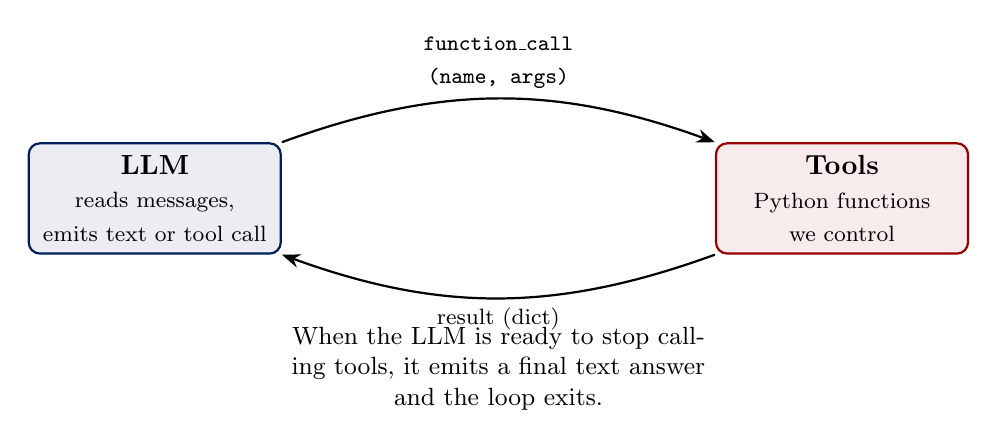
\begin{tikzpicture}[node distance=1.5cm, >=Stealth, thick]
    \node[rectangle, draw=pennblue, fill=pennblue!8, rounded corners, minimum width=3.2cm, minimum height=1.4cm, align=center] (llm) {\textbf{LLM}\\\footnotesize reads messages,\\\footnotesize emits text or tool call};
    \node[rectangle, draw=pennred, fill=pennred!8, rounded corners, minimum width=3.2cm, minimum height=1.4cm, align=center, right=5.5cm of llm] (tool) {\textbf{Tools}\\\footnotesize Python functions\\\footnotesize we control};

    \draw[->, thick] (llm.north east) to[bend left=20]
      node[above, midway, align=center] {\footnotesize \texttt{function\_call}\\\footnotesize \texttt{(name, args)}} (tool.north west);
    \draw[->, thick] (tool.south west) to[bend left=20]
      node[below, midway] {\footnotesize result (dict)} (llm.south east);

    \node[below=1.5cm of $(llm)!0.5!(tool)$, align=center, text width=10cm, font=\small]
      {When the LLM is ready to stop calling tools, it emits a final text answer\\ and the loop exits.};
  \end{tikzpicture}
\end{frame}

% ============================================================
\begin{frame}[fragile]{What a tool is}
  Two pieces, written by us: an ordinary Python function, and a JSON-schema description of its signature that we hand to the model.

  \vskip0.5em

  \begin{columns}[T]
  \column{0.42\textwidth}
  \textbf{\footnotesize Python function (we call it)}
\begin{lstlisting}
def calculator(op, a, b):
    ops = {"add": a+b, "sub": a-b,
           "mul": a*b, "div": a/b}
    return {"result": ops[op]}
\end{lstlisting}

  \column{0.55\textwidth}
  \textbf{\footnotesize JSON schema (the model reads it)}
\begin{lstlisting}
{
  "name": "calculator",
  "description": "One arithmetic op.",
  "parameters": {
    "type": "object",
    "properties": {
      "op": {"type": "string",
             "enum": ["add","sub","mul","div"]},
      "a":  {"type": "number"},
      "b":  {"type": "number"},
    },
    "required": ["op","a","b"],
  },
}
\end{lstlisting}
  \end{columns}

  \vskip0.4em

  What each schema field controls:
  \begin{itemize}
    \item \texttt{name}, \texttt{description} --- whether the model picks this tool over others.
    \item \texttt{parameters.properties} --- the typed argument list. \texttt{enum} restricts a string to a fixed set; \texttt{type} restricts to \texttt{string}/\texttt{number}/\texttt{integer}/\texttt{boolean}/\texttt{array}/\texttt{object}.
    \item \texttt{required} --- args the model must supply (the rest are optional).
  \end{itemize}
\end{frame}

% ============================================================
\begin{frame}[fragile]{Tool calling: the round trip}
  Each turn the model emits either plain text (final answer) or a structured tool call.

  \vskip0.5em

  \textbf{1. Model's reply contains a \texttt{function\_call} part:}
\begin{lstlisting}
response.candidates[0].content.parts[0].function_call
  .name = "calculator"
  .args = {"op": "mul", "a": 13, "b": 47}
\end{lstlisting}

  \textbf{2. We dispatch by name and run the Python function:}
\begin{lstlisting}
result = tool_fns[name](**args)   # = {"result": 611}
\end{lstlisting}

  \textbf{3. We send the result back as a \texttt{function\_response} on the next turn:}
\begin{lstlisting}
Part.from_function_response(name="calculator",
                            response={"result": 611})
\end{lstlisting}

  \vskip0.4em

  Loop: the model sees its own previous call, the result, and decides whether to call another tool or stop and return text.
\end{frame}

% ============================================================
\begin{frame}[fragile]{The ReAct loop in pseudocode}
\begin{lstlisting}
def run_agent(system_prompt, user_prompt, tool_schemas, tool_fns,
              max_steps=12):
    messages = [user_prompt]
    for step in range(max_steps):
        response = llm(system_prompt, messages, tools=tool_schemas)
        messages.append(response)
        if response.is_tool_call:
            for call in response.tool_calls:
                try:
                    result = tool_fns[call.name](**call.args)
                except Exception as e:
                    result = {"error": str(e)}
                messages.append(result)
        else:
            return response.text  # final answer
\end{lstlisting}
  The notebook has this, fleshed out, in about 30 lines.
\end{frame}

% ============================================================
\begin{frame}[fragile]{Two slots: \texttt{system\_prompt} vs \texttt{user\_prompt}}
  \texttt{run\_agent} takes two prompt strings and puts them in different slots:

  \vskip0.6em

  \begin{itemize}
    \item \textbf{\texttt{system\_prompt}} --- the \textit{rules of the game}. Identity, methodology, what the tools are for, budgets, how to stop. Sent on every turn as a persistent header; never gets drowned out as observations pile up.
    \item \textbf{\texttt{user\_prompt}} --- the \textit{specific ask} that triggers this run. Becomes the first message of the conversation; tool calls and observations append after it.
  \end{itemize}

  \vskip0.6em

  For example, the B1 optimization agent splits them like this:
\begin{lstlisting}
B1_SYSTEM = """You optimize a black-box function (angle in degrees,
in (0, 90)) returning a range in meters. Budget: at most 12 evaluate()
calls. Use history if helpful, then call propose_answer with your guess."""

B1_USER = "Find the optimal angle. Budget: 12 evaluations."
\end{lstlisting}

  \vskip0.3em

  Rule of thumb: durable rules about \textit{how to behave} go in \texttt{system\_prompt}; the specific \textit{thing to do this run} goes in \texttt{user\_prompt}.
\end{frame}

% ============================================================
\begin{frame}[fragile]{Errors are observations}
  Tool calls will sometimes fail: the model invents a nonexistent argument, asks for a mesh ID that doesn't exist, passes a string instead of a number.

  \vskip0.8em

  The loop wraps every dispatch in \texttt{try/except} and feeds the exception back as the tool's observation:

  \vskip0.5em
\begin{lstlisting}
try:
    result = tool_fns[name](**args)
except Exception as e:
    result = {"error": f"{type(e).__name__}: {e}"}
\end{lstlisting}

  \vskip0.5em

  The model reads the error on the next turn and, with a reasonable prompt, retries with correct arguments.

  \vskip0.5em
  \textcolor{codegray}{\small In the tutorial you will see this trigger in practice. Do not treat it as a bug.}
\end{frame}

% ============================================================
\begin{frame}{ReAct is the simplest option. Two others.}
  \begin{columns}[T]
  \column{0.48\textwidth}
    \textbf{Multi-agent} (LangGraph, AutoGen, CrewAI)

    \vskip0.4em

    A state machine of specialized agents. Each node is an LLM with its own system prompt and tool subset; edges encode control flow.

    \vskip0.6em
    \centering
    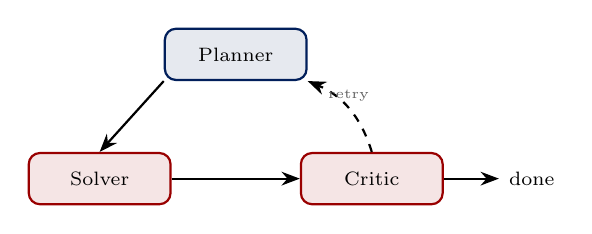
\begin{tikzpicture}[>=Stealth, thick, font=\scriptsize]
      \node[draw=pennblue, fill=pennblue!10, rounded corners, minimum width=1.8cm, minimum height=0.65cm] (p) {Planner};
      \node[draw=pennred, fill=pennred!10, rounded corners, minimum width=1.8cm, minimum height=0.65cm, below left=0.9cm and -0.1cm of p] (w) {Solver};
      \node[draw=pennred, fill=pennred!10, rounded corners, minimum width=1.8cm, minimum height=0.65cm, below right=0.9cm and -0.1cm of p] (c) {Critic};
      \draw[->] (p.south west) -- (w.north);
      \draw[->] (w.east) -- (c.west);
      \draw[->, dashed] (c.north) to[bend right=25] node[above, font=\tiny, text=codegray, yshift=-0.1em]{retry} (p.south east);
      \draw[->] (c.east) -- ++(0.7,0) node[right, font=\scriptsize] {done};
    \end{tikzpicture}
    \vskip0.6em

    \textbf{Beats ReAct when} roles are genuinely distinct, branches run in parallel, or each role needs its own guardrails.

  \column{0.48\textwidth}
    \textbf{MPC-style} (Model Predictive Control)

    \vskip0.4em

    At each step: look ahead, plan the next $N$ actions against a world model, execute only the first action, then re-plan. Tree-of-Thoughts is a related variant that searches branches.

    \vskip0.6em
    \centering
    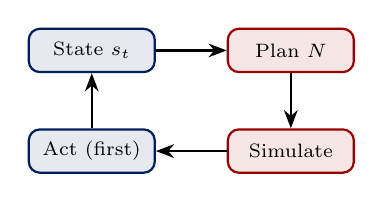
\begin{tikzpicture}[>=Stealth, thick, font=\scriptsize]
      \node[draw=pennblue, fill=pennblue!10, rounded corners, minimum width=1.6cm, minimum height=0.55cm] (s) {State $s_t$};
      \node[draw=pennred, fill=pennred!10, rounded corners, minimum width=1.6cm, minimum height=0.55cm, right=0.9cm of s] (pl) {Plan $N$};
      \node[draw=pennred, fill=pennred!10, rounded corners, minimum width=1.6cm, minimum height=0.55cm, below=0.7cm of pl] (si) {Simulate};
      \node[draw=pennblue, fill=pennblue!10, rounded corners, minimum width=1.6cm, minimum height=0.55cm, below=0.7cm of s] (ac) {Act (first)};
      \draw[->] (s) -- (pl);
      \draw[->] (pl) -- (si);
      \draw[->] (si) -- (ac);
      \draw[->] (ac) -- (s);
    \end{tikzpicture}
    \vskip0.6em

    \textbf{Beats ReAct when} the cost of a wrong action is high and you have a cheap, trusted forward simulator or world model.
  \end{columns}
\end{frame}

% ============================================================
\section*{Part 2: Adaptive FEM}

\begin{frame}{Task 1: adaptive mesh refinement on an L-shape}
  \begin{columns}[T]
  \column{0.55\textwidth}
    Poisson with uniform forcing:
    \[
      -\Delta u = 1 \ \text{in } \Omega, \qquad u = 0 \ \text{on } \partial\Omega.
    \]

    The re-entrant corner at the origin gives a singular solution
    \[
      u \sim r^{2/3} \sin(2\theta/3)
    \]
    so $u \in H^{5/3-\epsilon}$, $u \notin H^2$.

    \vskip0.8em

    \textbf{Task for the agent:} drive the $H^1$ error below a tolerance by choosing where to refine.

  \column{0.45\textwidth}
    \centering
    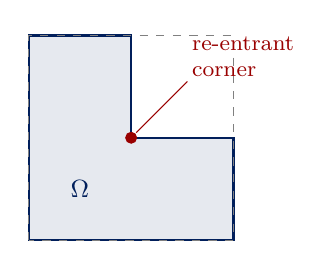
\begin{tikzpicture}[scale=1.3]
      \filldraw[fill=pennblue!10, draw=pennblue, thick]
        (1,0) -- (1,-1) -- (-1,-1) -- (-1,1) -- (0,1) -- (0,0) -- cycle;
      \draw[dashed, gray] (-1,-1) rectangle (1,1);
      \filldraw[pennred] (0,0) circle (1.5pt);
      \draw[pennred, thin] (0.05,0.05) -- (0.55,0.55);
      \node[anchor=south west, pennred, font=\footnotesize, align=left] at (0.5,0.5) {re-entrant\\corner};
      \node[anchor=center, font=\small, pennblue] at (-0.5,-0.5) {$\Omega$};
    \end{tikzpicture}
  \end{columns}
\end{frame}

% ============================================================
\begin{frame}{Expected convergence}
  P1 finite elements:
  \begin{itemize}
    \item \textbf{Uniform refinement.} Asymptotic $H^1$-seminorm rate is $O(h^{2/3})$. Pre-asymptotically you will often see rates of 0.7 to 0.95.
    \item \textbf{Adaptive refinement} (driven by a local error indicator). Optimal rate $O(N^{-1/2})$, i.e.\ rate 1 against $h \sim N^{-1/2}$.
  \end{itemize}

  \vskip1em

  The gap between these two rates is the entire point of adaptive meshing on this problem. We will make the agent rediscover it.
\end{frame}

% ============================================================
\begin{frame}{What ``adaptive refinement'' actually means}
  \textbf{1. A local error indicator $\eta_K$.} For each element $K$, a computable proxy for how much error lives there. We use the \textit{gradient-jump indicator}:
  \[
    \eta_K^2 \;=\; \tfrac{1}{2}\!\sum_{e \,\in\, \partial K \cap \Omega^{\circ}} h_e \, \big| [\![\nabla u_h \cdot n_e]\!] \big|^2.
  \]
  P1 elements have discontinuous gradients across element edges, and the size of the jump correlates with the local error.

  \vskip0.6em

  \textbf{2. D\"orfler marking.} Pick a bulk fraction $\theta \in (0,1)$. Mark the smallest set of elements $\mathcal{M}$ whose squared indicators capture a fraction $\theta$ of the total:
  \[
    \sum_{K \in \mathcal{M}} \eta_K^2 \;\ge\; \theta \sum_{K} \eta_K^2.
  \]
  Refine those; leave the rest. In practice: sort elements by $\eta_K$ descending, walk down the list until the running sum hits $\theta \cdot \text{total}$, refine everything you walked past.

  \vskip0.4em

  \textcolor{codegray}{\small $\theta = 0.5$ is the textbook default. Smaller $\theta$ = focus on the worst offenders (slower mesh growth). Larger $\theta$ = closer to uniform refinement.}
\end{frame}

% ============================================================
\begin{frame}{Tools the FEM agent gets}
  Each tool takes a \texttt{mesh\_id} (integer) and returns a dict.
  \vskip0.3em
  \begin{itemize}
    \item \texttt{solve\_poisson(mesh\_id)} $\to$ \{dofs, $H^1$ error\}
    \item \texttt{local\_indicators(mesh\_id)} $\to$ per-element gradient-jump indicators (summary stats)
    \item \texttt{uniform\_refine(mesh\_id)} $\to$ new mesh id
    \item \texttt{refine\_by\_threshold(mesh\_id, theta)} $\to$ Dorfler-mark and refine
    \item \texttt{check\_convergence\_rate()} $\to$ log-log slope of last 3 solves vs theory
    \item \texttt{stop(reason)}
  \end{itemize}

  \vskip0.8em

  Guardrails built in: \texttt{MAX\_DOFS = 20000}; every tool is \texttt{try/except}-wrapped.
\end{frame}

% ============================================================
\begin{frame}{Three prompts you will write}
  \textbf{A1.} Uniform refinement agent. Only allowed to use \texttt{uniform\_refine}.

  \vskip0.5em
  \textbf{A2.} Adaptive refinement agent. Uses \texttt{refine\_by\_threshold} with Dorfler marking ($\theta = 0.5$).

  \vskip0.5em
  \textbf{A3.} Rate-checking agent. Calls \texttt{check\_convergence\_rate} every cycle and adapts $\theta$ if the empirical rate drops.

  \vskip1em

  Plot at the end: $H^1$ error vs $h \sim 1/\sqrt{N}$ on log-log, all three agents overlaid, with theoretical slopes $2/3$ and $1$.
\end{frame}

% ============================================================
\section*{Part 3: Black-box optimization}

\begin{frame}{Task 2: projectile with drag}
  Quadratic drag:
  \[
    \ddot{x} = -c_d |v|\, \dot{x}, \qquad \ddot{y} = -g - c_d |v|\, \dot{y}.
  \]
  Parameters: $v_0 = 50$~m/s, $c_d = 0.01$~m$^{-1}$, $g = 9.81$~m/s$^2$.

  \vskip1em

  \textbf{Task for the agent:} find the launch angle $\theta \in (0^\circ, 90^\circ)$ that maximizes horizontal range.

  \vskip0.8em

  Without drag the optimum is $45^\circ$; with drag it shifts lower. The agent does not see the ODE; it only sees the outputs of a black-box \texttt{evaluate(angle)} tool.
\end{frame}

% ============================================================
\begin{frame}{Tools the optimization agent gets}
  \begin{itemize}
    \item \texttt{evaluate(angle\_deg)} $\to$ horizontal range (m)
    \item \texttt{history()} $\to$ all past (angle, range) evaluations
    \item \texttt{propose\_answer(angle\_deg, rationale)} $\to$ final guess
    \item (bonus) \texttt{evaluate\_height(angle\_deg)} $\to$ max altitude
  \end{itemize}

  \vskip0.8em

  \textbf{Three prompts you will write:}
  \begin{itemize}
    \item \textbf{B1.} Trial agent. Small budget, any search strategy.
    \item \textbf{B2.} Finite-difference gradient agent. Centered FD estimate of $dR/d\theta$, step in the ascent direction. Callback to Lecture 3.
    \item \textbf{B3} (bonus). Maximize range subject to $\max_t y(t) \le 30$~m.
  \end{itemize}
\end{frame}

% ============================================================
\section*{Verifiers}

\begin{frame}{The verifier-agent pattern}
  After each of the two main tasks, we run a \textbf{second, separate agent} that does not trust the first:

  \vskip0.8em

  \begin{itemize}
    \item \textbf{Part 2 verifier.} Designs its own manufactured-solution test. Picks a smooth $u_{\text{exact}}$, computes $f = -\Delta u_{\text{exact}}$, solves with $u_h = u_{\text{exact}}$ on $\partial\Omega$, and checks the errors converge at the expected rates.
    \item \textbf{Part 3 verifier.} Takes the claimed optimal angle and re-integrates the ODE with \texttt{solve\_ivp(method="RK45", rtol=1e-10)}. Reports the discrepancy against \texttt{odeint}.
  \end{itemize}

  \vskip0.8em

  A verifier is just another agent with a different system prompt and a different tool set.
\end{frame}

% ============================================================
\section*{Logistics}

\begin{frame}{Before we start}
  \begin{enumerate}
    \item Get a free Gemini API key at \texttt{aistudio.google.com/apikey}. Sign in with any Google account.
    \item Open the Colab notebook (linked on the course page, Apr 27).
    \item In Colab, click the \textit{Secrets} panel (key icon, left sidebar) and add a secret named \texttt{GEMINI\_API\_KEY} with your key as the value.
    \item Run the Part 0 cells to confirm the client connects.
  \end{enumerate}

  \vskip1em

  \textcolor{codegray}{\small If you already have an Anthropic, OpenAI, or Groq key you can swap backends by editing a few lines in the \texttt{run\_agent} function (noted in the notebook).}
\end{frame}

% ============================================================
\begin{frame}[plain]
  \vfill
  \centering
  {\Huge\bfseries\color{pennblue} Let's go.}\\[2em]
  {\color{codegray}\small Open the notebook and run Part 0.}
  \vfill
\end{frame}

\end{document}
